\section{Exercise 4}
Using python build an user defined subroutine to compute the $QR$
factorization for a square matrix $A$ with the provided pseudo code. Verify
your subroutine works by factoring the following matrix $A$ and printing
$Q$, $R$, and $A-QR$.

\begin{equation}
  A =
  \begin{bmatrix}
    12  &  -51   &  4   \\
    6   &  167   &  -68   \\
    -4  &  24    &  -41
  \end{bmatrix}
\end{equation}

Next, compare the performance of your $QR$ factorization to the $LU$
factorization coded in Assignment 1 (use the solution from Assignment 1 if
you were unable to get the $LU$ factorization tool working) using $N = 10,
100, 500, 1000, 2000$.
\begin{mdframed}[style=MyFrame]
    We start by performing the verification case which should have
    produced the following, 
    \begin{equation}
        A = 
        \underbrace{
        \begin{bmatrix}
            0.85714     &    -0.39429       &   -0.33143    \\
            0.42857     &    0.90286        &    0.03429    \\
            -0.28571    &    0.17143        &  -0.94286
        \end{bmatrix}
        }_{\equiv Q}
        \underbrace{
        \begin{bmatrix}
            14      &   21      &           -14         \\
            0       &   175     &           -70         \\
            0       &   0       &           35
        \end{bmatrix}
        }_{\equiv R}
    \end{equation}
    Comparing the time requirement between $LU$ and $QR$ we see from
    Fig~(\ref{fig:QR-LU}) that $LU$ is significantly faster compared to
    $QR$. This should not be surprising given the added number of flops
    needed to perform the projection, normalize $Q$, and find $R$ compared
    to simple row operations.
    \begin{figure}[H]
        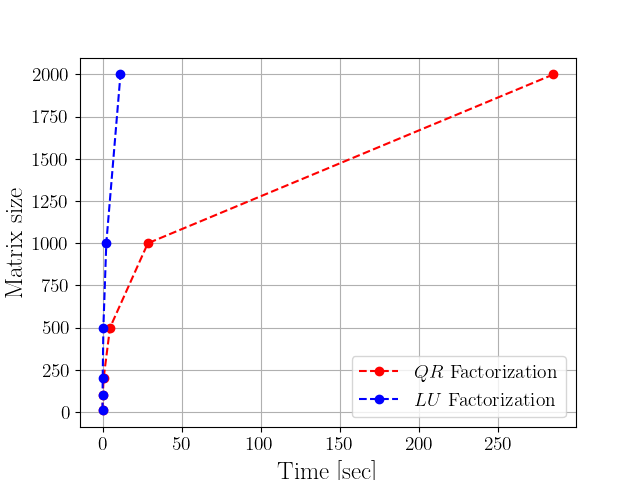
\includegraphics[height=0.35\textheight]{../media/QR-LU.png}
        \caption{Comparison between the $QR$ and $LU$ factorization}
        \label{fig:QR-LU}
    \end{figure}

\end{mdframed}
